\documentclass[aspectratio=169,10pt]{beamer}

\usetheme{default}
\usecolortheme{default}
\setbeamertemplate{navigation symbols}{}
\setbeamertemplate{footline}[frame number]

\usepackage[T1]{fontenc}
\usepackage{amsmath,booktabs}
\usepackage[dvipsnames]{xcolor}
\usepackage{tikz}
\usetikzlibrary{arrows.meta,positioning}

\definecolor{accent}{RGB}{25,90,150}
\setbeamercolor{structure}{fg=accent}
\setbeamercolor{frametitle}{fg=accent}

\title{Embedding-Aware Cooperative LiDAR Perception}
\subtitle{Spatial TrackFormer Association and SWFormer Detector Exploration}
\author{Dhia}
\date{July 2026}

\begin{document}

\begin{frame}
  \titlepage
  \vfill
  \centering\small
  TrackFormer~\cite{trackformer} is adapted from temporal tracking to
  same-timestamp cross-agent association in OPV2V.
\end{frame}

\begin{frame}{What We Built}
\begin{columns}[T,onlytextwidth]
\column{0.49\textwidth}
\begin{block}{Detector and data}
\begin{itemize}
  \item OpenCOOD PointPillars runs on the target hardware.
  \item Clean late fusion reproduces $\mathrm{AP@0.7}\approx0.78$.
  \item We cache detections, identities, confidence, box geometry, and every
  vehicle-covered BEV feature cell.
\end{itemize}
\end{block}

\column{0.49\textwidth}
\begin{block}{Association objective}
\begin{itemize}
  \item Given a source-agent detection and an ego-agent detection at the
  same timestamp, decide whether they are the same physical vehicle.
  \item Transform box geometry into the ego frame before comparison.
  \item Output a normalized 128-D association embedding per proposal.
\end{itemize}
\end{block}
\end{columns}

\vspace{3mm}
\centering
\alert{Key correction:} the original MLP read only one BEV feature cell;
the final model reads all cells covered by the vehicle box.
\end{frame}

\begin{frame}{SWFormer: Why Use a Sparse-Window Transformer?}
\begin{columns}[T,onlytextwidth]
\column{0.48\textwidth}
\begin{block}{The LiDAR problem}
\begin{itemize}\setlength{\itemsep}{3pt}
  \item A driving scene spans a large ground-plane area, but only a small
  fraction of cells contain LiDAR points.
  \item A dense BEV CNN still computes over many empty cells; global attention
  over all cells would be prohibitively expensive.
\end{itemize}
\end{block}

\column{0.48\textwidth}
\begin{block}{SWFormer contribution~\cite{swformer}}
\begin{itemize}\setlength{\itemsep}{3pt}
  \item Keep only occupied voxels as sparse tokens.
  \item Apply self-attention inside small spatial windows, then shift windows
  so neighbouring regions can exchange information.
  \item Fuse multiple sparse resolutions and diffuse foreground information
  before predicting object centers and boxes.
\end{itemize}
\end{block}
\end{columns}

\vspace{3mm}
\centering
\alert{High-level goal:} obtain Transformer context without paying for dense
computation over empty LiDAR space.
\end{frame}

\begin{frame}{SWFormer Detector Architecture: One CAV, One LiDAR Sweep}
\centering
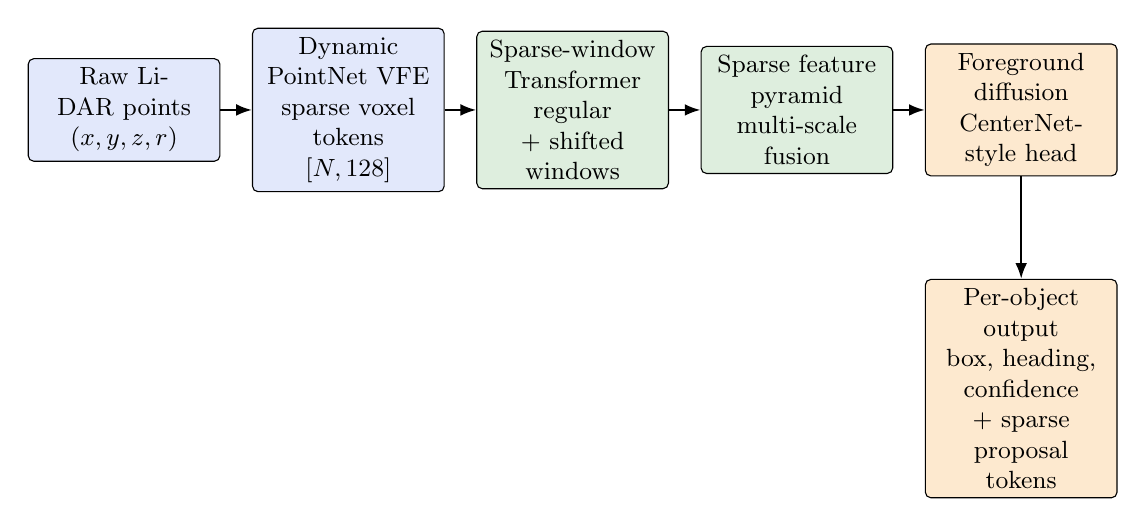
\begin{tikzpicture}[
  font=\small,
  box/.style={draw, rounded corners=2pt, align=center, minimum height=10mm,
    text width=22mm},
  bluebox/.style={box, fill=RoyalBlue!15},
  greenbox/.style={box, fill=ForestGreen!15},
  orangebox/.style={box, fill=BurntOrange!16},
  arrow/.style={-{Latex[length=2mm]}, thick},
  node distance=4mm
]
\node[bluebox] (points) {Raw LiDAR points\\$(x,y,z,r)$};
\node[bluebox,right=of points] (vfe) {Dynamic PointNet VFE\\sparse voxel tokens\\$[N,128]$};
\node[greenbox,right=of vfe] (window) {Sparse-window Transformer\\regular + shifted windows};
\node[greenbox,right=of window] (pyramid) {Sparse feature pyramid\\multi-scale fusion};
\node[orangebox,right=of pyramid] (head) {Foreground diffusion\\CenterNet-style head};

\node[orangebox,below=13mm of head] (out) {Per-object output\\box, heading, confidence\\+ sparse proposal tokens};

\draw[arrow] (points) -- (vfe);
\draw[arrow] (vfe) -- (window);
\draw[arrow] (window) -- (pyramid);
\draw[arrow] (pyramid) -- (head);
\draw[arrow] (head) -- (out);
\end{tikzpicture}

\vspace{1mm}
\scriptsize
\begin{itemize}\setlength{\itemsep}{2pt}
  \item A \textbf{window} is a local $10\times10$ BEV neighbourhood; attention
  compares occupied tokens only within that window. Shifted windows connect
  neighbouring windows on the next block.
  \item The feature pyramid provides both fine spatial detail and broader
  scene context. Voxel diffusion supplies nearby context where LiDAR points
  are sparse around an object.
  \item Our current OpenCOOD experiment uses one sweep per CAV; it does not
  yet exploit SWFormer's optional multi-sweep temporal input.
\end{itemize}
\end{frame}

\begin{frame}{How SWFormer Learns 3D Detection}
\small
For each sparse BEV token, SWFormer predicts foreground, an object-center
heatmap, box parameters, and heading. The implemented objective is
\[
\mathcal{L}_{\mathrm{SW}}=
200\,\mathcal{L}_{\mathrm{seg}}^{\mathrm{focal}}+
10\,\mathcal{L}_{\mathrm{center}}^{\mathrm{focal}}+
\mathcal{L}_{\mathrm{box}}^{\mathrm{Smooth}\text{-}L_1}+
\mathcal{L}_{\mathrm{heading}}^{\mathrm{CE}+\mathrm{Smooth}\text{-}L_1}+
\mathcal{L}_{\mathrm{IoU}}^{3\mathrm{D}}.
\]

\begin{columns}[T,onlytextwidth]
\column{0.49\textwidth}
\begin{itemize}\setlength{\itemsep}{4pt}
  \item $\mathcal{L}_{\mathrm{seg}}$: classify sparse cells as foreground or
  background; focal weighting handles the large background majority.
  \item $\mathcal{L}_{\mathrm{center}}$: make each vehicle center a confident
  local heatmap peak.
  \item $\mathcal{L}_{\mathrm{box}}$: regress center offsets and $h,w,l$.
\end{itemize}

\column{0.49\textwidth}
\begin{itemize}\setlength{\itemsep}{4pt}
  \item $\mathcal{L}_{\mathrm{heading}}$: classify one of 12 yaw bins and
  regress the residual within that bin.
  \item $\mathcal{L}_{\mathrm{IoU}}^{3\mathrm{D}}$: directly rewards overlap
  between the decoded oriented prediction and its ground-truth box.
  \item The final confidence score is used to rank detections for the
  precision--recall curve and AP.
\end{itemize}
\end{columns}

\vspace{2mm}
\centering\footnotesize
\alert{Important:} lower training loss is useful, but validation AP measures
the actual detection-and-ranking quality we report.
\end{frame}

\begin{frame}{Detector Features $\rightarrow$ Shared Embedding Interface}
\centering
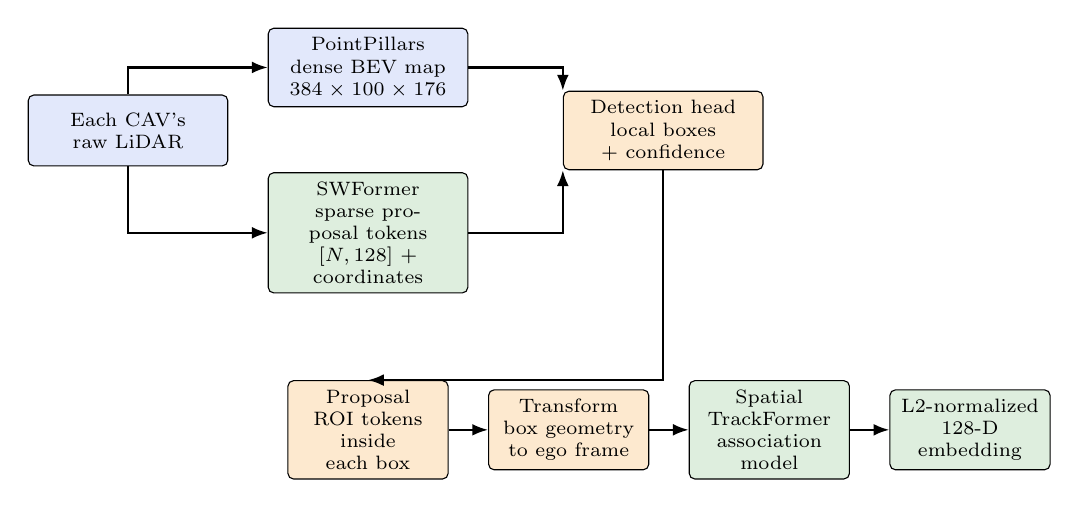
\begin{tikzpicture}[
  font=\scriptsize,
  box/.style={draw, rounded corners=2pt, align=center, minimum height=9mm,
    text width=23mm},
  smallbox/.style={box, text width=18mm},
  bluebox/.style={box, fill=RoyalBlue!15},
  greenbox/.style={box, fill=ForestGreen!15},
  orangebox/.style={box, fill=BurntOrange!16},
  arrow/.style={-{Latex[length=2mm]}, thick},
  node distance=4mm and 5mm
]
\node[bluebox] (lidar) {Each CAV's\\raw LiDAR};
\node[bluebox,right=of lidar,yshift=8mm] (pp) {PointPillars\\dense BEV map\\$384\times100\times176$};
\node[greenbox,right=of lidar,yshift=-13mm] (sw) {SWFormer\\sparse proposal tokens\\$[N,128]$ + coordinates};
\node[orangebox,right=12mm of pp,yshift=-8mm] (detect) {Detection head\\local boxes + confidence};
\node[orangebox,smallbox,below=11mm of sw] (roi) {Proposal ROI tokens\\inside each box};
\node[orangebox,smallbox,right=of roi] (ego) {Transform box geometry\\to ego frame};
\node[greenbox,smallbox,right=of ego] (assoc) {Spatial TrackFormer\\association model};
\node[greenbox,smallbox,right=of assoc] (embed) {L2-normalized\\128-D embedding};

\draw[arrow] (lidar) |- (pp.west);
\draw[arrow] (lidar) |- (sw.west);
\draw[arrow] (pp.east) -| (detect.north west);
\draw[arrow] (sw.east) -| (detect.south west);
\draw[arrow] (detect.south) |- (roi.north);
\draw[arrow] (roi) -- (ego);
\draw[arrow] (ego) -- (assoc);
\draw[arrow] (assoc) -- (embed);
\end{tikzpicture}

\vspace{0mm}
\scriptsize
\begin{itemize}\setlength{\itemsep}{1pt}
  \item \textbf{Shared contract:} whichever detector is used, it supplies a
  detected box, confidence, and the proposal-aligned feature tokens inside
  that object region.
  \item The source and ego boxes are represented in the same ego coordinate
  frame before association. Spatial TrackFormer then maps object evidence to a
  128-D vector; similar vectors support cross-agent grouping.
  \item PointPillars currently supplies the trained embedding cache. SWFormer
  now exposes its native sparse proposal tokens, enabling the same downstream
  association interface in a future experiment.
\end{itemize}
\end{frame}

\begin{frame}{From LiDAR Points to an Object Embedding}
\centering
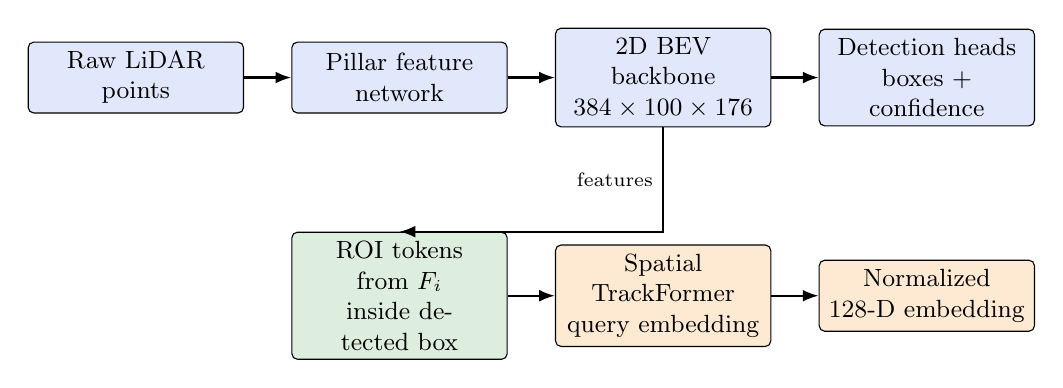
\begin{tikzpicture}[
  font=\small,
  box/.style={draw, rounded corners=2pt, align=center, minimum height=9mm,
    text width=25mm},
  bluebox/.style={box, fill=RoyalBlue!15},
  greenbox/.style={box, fill=ForestGreen!15},
  orangebox/.style={box, fill=BurntOrange!15},
  arrow/.style={-{Latex[length=2mm]}, thick},
  node distance=6mm
]
\node[bluebox] (points) {Raw LiDAR\\points};
\node[bluebox,right=of points] (pillar) {Pillar feature\\network};
\node[bluebox,right=of pillar] (bev) {2D BEV backbone\\$384\times100\times176$};
\node[bluebox,right=of bev] (heads) {Detection heads\\boxes + confidence};

\node[greenbox,below=15mm of pillar] (roi) {ROI tokens from $F_i$\\inside detected box};
\node[orangebox,right=of roi] (trackformer) {Spatial TrackFormer\\query embedding};
\node[orangebox,right=of trackformer] (embed) {Normalized\\128-D embedding};

\draw[arrow] (points) -- (pillar);
\draw[arrow] (pillar) -- (bev);
\draw[arrow] (bev) -- (heads);
\draw[arrow] (bev.south) |- node[pos=0.25,left,font=\scriptsize]{features} (roi.north);
\draw[arrow] (roi) -- (trackformer);
\draw[arrow] (trackformer) -- (embed);
\end{tikzpicture}

\vspace{1mm}
{\footnotesize
\begin{itemize}\setlength{\itemsep}{1pt}
  \item \textbf{Pillar feature network:} a point-wise MLP and max pooling
  convert all points in one vertical XY cell into one learned pillar descriptor.
  \item \textbf{2D BEV backbone:} a CNN scatters these descriptors onto the
  ground plane and combines neighbouring pillars into contextual features.
  \item $384$ is the number of learned channels, \emph{not} the number or size
  of pillars; $100\times176$ is the final spatial grid after the backbone's
  strides, starting from the configured LiDAR range and $0.4\,$m voxel grid.
  \item \textbf{Detection heads} are small convolutional layers that predict a
  vehicle score and box offsets at every BEV location/anchor. \textbf{ROI}
  means \emph{Region of Interest}: the 6--21 BEV cells covered by that box.
\end{itemize}
}
\end{frame}

\begin{frame}{TrackFormer Training: Temporal Tracking $\rightarrow$ Spatial Association}
\begin{columns}[T,onlytextwidth]
\column{0.48\textwidth}
\textbf{Original TrackFormer}\par\vspace{1mm}
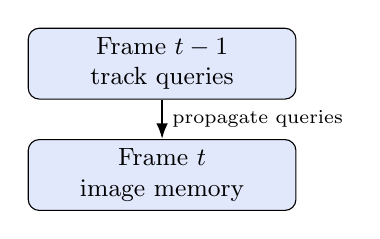
\begin{tikzpicture}[
  font=\small,
  q/.style={draw, rounded corners, fill=RoyalBlue!15, align=center,
  minimum width=34mm, minimum height=9mm},
  arrow/.style={-{Latex[length=2mm]}, thick}, node distance=5mm]
\node[q] (tminus) {Frame $t-1$\\track queries};
\node[q,below=of tminus] (t) {Frame $t$\\image memory};
\draw[arrow] (tminus) -- node[right,font=\scriptsize]{propagate queries} (t);
\end{tikzpicture}

\vspace{1mm}\footnotesize
Frame $t-1$ detections spawn queries that carry identity into frame $t$.

\column{0.52\textwidth}
\textbf{Our spatial adaptation}\par\vspace{1mm}
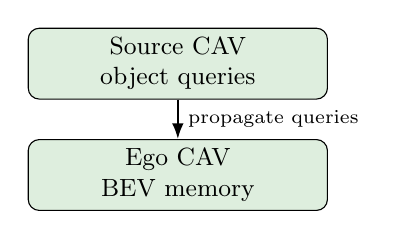
\begin{tikzpicture}[
  font=\small,
  q/.style={draw, rounded corners, fill=ForestGreen!15, align=center,
  minimum width=38mm, minimum height=9mm},
  arrow/.style={-{Latex[length=2mm]}, thick}, node distance=5mm]
\node[q] (source) {Source CAV\\object queries};
\node[q,below=of source] (ego) {Ego CAV\\BEV memory};
\draw[arrow] (source) -- node[right,font=\scriptsize]{propagate queries} (ego);
\end{tikzpicture}

\vspace{1mm}\footnotesize
Source-CAV detections spawn queries that attend to ego-CAV BEV memory at the
same timestamp.
\end{columns}

\vspace{2mm}
\footnotesize
\textbf{Training objective from the TrackFormer paper.} New objects use
Hungarian matching; persistent tracks are matched by their known identity:
\[
  \hat\sigma=\arg\min_{\sigma}\sum_i
  \left[-\lambda_{\mathrm{cls}}\hat p_{\sigma(i)}(c_i)+C_{\mathrm{box}}(b_i,\hat b_{\sigma(i)})\right],
  \qquad C_{\mathrm{box}}=\lambda_1\|b_i-\hat b_{\sigma(i)}\|_1+
  \lambda_{\mathrm{giou}}C_{\mathrm{giou}}.
\]
\[
 \mathcal{L}_{\mathrm{MOT}}=\sum_j\left[
 \mathrm{CE}(c_j,\hat p_j)+\mathbb{1}_{j\in\pi}
 \bigl(\lambda_1\mathcal{L}_1+\lambda_{\mathrm{giou}}\mathcal{L}_{\mathrm{giou}}\bigr)\right],
 \quad c_j=0\ \text{for unmatched queries}.
\]
\centering\footnotesize\alert{Why this can work:} source queries attend to ego
BEV memory; shared-frame geometry disambiguates similar vehicles. False
negative and false positive queries teach recovery and rejection.
\end{frame}

\begin{frame}{Exact Cross-Agent TrackFormer Pipeline}
\footnotesize
For source agent $i$: $F_i\in\mathbb{R}^{384\times100\times176}$ is its
local BEV map and $P_i=\{(b^{\mathrm{local}}_{i,k},s_{i,k})\}$ are its
local detected boxes and confidence scores.

\begin{block}{Definitions: one proposal $k$ from source agent $i$}
\begin{itemize}\setlength{\itemsep}{1pt}
  \item $\mathcal{R}_{i,k}$: \textbf{index set} of BEV cells covered by the
  rotated detected box $b_{i,k}$; it is not a feature vector.
  \item $X_{i,k}=[F_i(r_1);\ldots;F_i(r_m)]\in\mathbb{R}^{m\times384}$:
  the actual \textbf{ROI token data} selected from $F_i$ using $\mathcal{R}_{i,k}$,
  with $m\approx6$--$21$ cells.
  \item $g_{i,k}\in\mathbb{R}^{9}$: the normalized ego-frame geometry and
  confidence $[x_e,y_e,z_e,h,w,l,\sin\psi,\cos\psi,s_{i,k}]$.
  \item $h_{i,k}\in\mathbb{R}^{256}$: learned final decoder \textbf{query
  state}; an internal float vector, not a box or raw LiDAR data.
  \item $z_{i,k}\in\mathbb{R}^{128}$: the L2-normalized \textbf{association
  embedding} computed from $h_{i,k}$ and $g_{i,k}$.
\end{itemize}
\end{block}

\begin{block}{Process and communication}
\textbf{Source:} $F_i,P_i\rightarrow\mathcal{R}_{i,k},X_{i,k},g_{i,k}
\rightarrow$ TrackFormer $\rightarrow(h_{i,k},z_{i,k})$; send selected query
states, ego-frame boxes, scores, and embeddings---not the full $F_i$ map.\\
\textbf{Ego:} builds $X_{e,k},g_{e,k}$, propagates received $h_{i,k}$ through
its BEV memory, then associates source and ego proposals. The detection head
defines each ROI and explicitly conditions TrackFormer through $g_{i,k}$.
\end{block}
\end{frame}

\begin{frame}{Embedding Results and Current Conclusion}
\centering
\begin{tabular}{lr}
\toprule
Model / evaluation & Top-1 association accuracy \\
\midrule
Single-cell MLP, held-out cache & $\approx0.21$ \\
Spatial TrackFormer + geometry head, clean validation & $0.915$ \\
Spatial TrackFormer + geometry head, clean OPV2V test & $0.891$ \\
Same clean model, noisy validation & $0.907$ \\
Same clean model, noisy OPV2V test & $0.891$ \\
\bottomrule
\end{tabular}

\vspace{5mm}
\begin{block}{Takeaway}
Using all vehicle-covered BEV cells and spatial TrackFormer query propagation
substantially improves cross-agent identity association. The embedding model
is strong in isolation; the remaining work is to translate this association
quality into better end-to-end fusion recall under noisy geometry.
\end{block}

\vfill
\scriptsize
\begin{thebibliography}{1}
\bibitem{trackformer} T.~Meinhardt et al., ``TrackFormer: Multi-Object
Tracking with Transformers,'' CVPR, 2022.
\bibitem{swformer} P.~Sun et al., ``SWFormer: Sparse Window Transformer for
3D Object Detection in Point Clouds,'' ECCV, 2022.
\end{thebibliography}
\end{frame}

\end{document}
